\documentclass[tikz,border=6pt]{standalone}
\usepackage[T1]{fontenc}
\usepackage{lmodern}
\usepackage{tikz}
\usetikzlibrary{arrows.meta,positioning}

\definecolor{bluehead}{HTML}{0789BB}
\definecolor{greenhead}{HTML}{008C4A}
\definecolor{brownhead}{HTML}{512900}
\definecolor{bluepanel}{HTML}{E7F4FE}
\definecolor{greenpanel}{HTML}{E8F8EF}
\definecolor{meshpanel}{HTML}{FAECFB}
\definecolor{dashpanel}{HTML}{E5ECFF}

\tikzset{
  >={Stealth[length=2mm]},
  box/.style={draw=black!55, line width=.7pt, rounded corners=3mm, fill=white},
  service/.style={box, minimum width=6.05cm, minimum height=1.00cm, align=center},
  tag/.style={fill=white, draw=black!25, rounded corners=1pt, inner sep=1.2pt, font=\scriptsize\bfseries},
  arrow/.style={->, draw=black!75, line width=.8pt}
}

\begin{document}
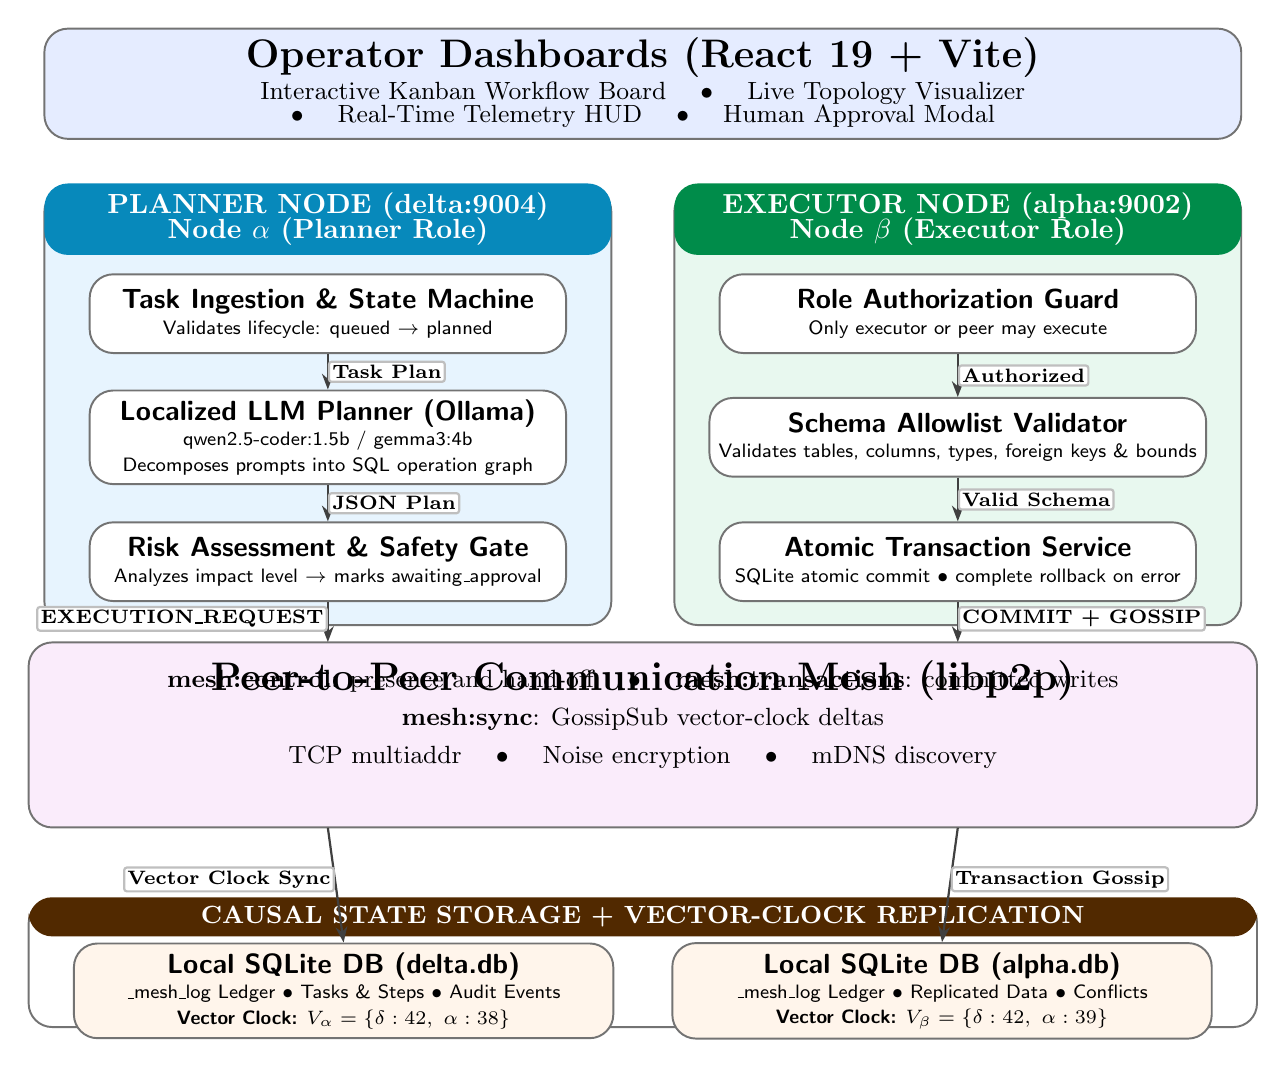
\begin{tikzpicture}[x=1cm,y=1cm,font=\sffamily]

% Dashboard
\node[box, fill=dashpanel, minimum width=15.2cm, minimum height=1.40cm] (dash) at (8,13.25) {};
\node[font=\bfseries\Large] at (8,13.58) {Operator Dashboards (React 19 + Vite)};
\node[font=\small,align=center] at (8,12.98)
  {Interactive Kanban Workflow Board \quad $\bullet$ \quad Live Topology Visualizer\\[-1mm]
   $\bullet$ \quad Real-Time Telemetry HUD \quad $\bullet$ \quad Human Approval Modal};

% Planner panel
\node[box, fill=bluepanel, minimum width=7.20cm, minimum height=5.55cm] (planner) at (4,9.15) {};
\node[fill=bluehead, rounded corners=3mm, minimum width=7.20cm, minimum height=.80cm,
      text=white, align=center, font=\bfseries] at (4,11.53)
  {PLANNER NODE (delta:9004)\\[-1mm] Node $\alpha$ (Planner Role)};
\node[service] (ingest) at (4,10.33) {\textbf{Task Ingestion \& State Machine}\\[-1mm]
  \scriptsize Validates lifecycle: queued $\rightarrow$ planned};
\node[service] (llm) at (4,8.76) {\textbf{Localized LLM Planner (Ollama)}\\[-1mm]
  \scriptsize qwen2.5-coder:1.5b / gemma3:4b\\[-1mm]
  \scriptsize Decomposes prompts into SQL operation graph};
\node[service] (risk) at (4,7.18) {\textbf{Risk Assessment \& Safety Gate}\\[-1mm]
  \scriptsize Analyzes impact level $\rightarrow$ marks awaiting\_approval};
\draw[arrow] (ingest.south) -- node[tag,right] {Task Plan} (llm.north);
\draw[arrow] (llm.south) -- node[tag,right] {JSON Plan} (risk.north);

% Executor panel
\node[box, fill=greenpanel, minimum width=7.20cm, minimum height=5.55cm] (executor) at (12,9.15) {};
\node[fill=greenhead, rounded corners=3mm, minimum width=7.20cm, minimum height=.80cm,
      text=white, align=center, font=\bfseries] at (12,11.53)
  {EXECUTOR NODE (alpha:9002)\\[-1mm] Node $\beta$ (Executor Role)};
\node[service] (guard) at (12,10.33) {\textbf{Role Authorization Guard}\\[-1mm]
  \scriptsize Only executor or peer may execute};
\node[service] (validate) at (12,8.76) {\textbf{Schema Allowlist Validator}\\[-1mm]
  \scriptsize Validates tables, columns, types, foreign keys \& bounds};
\node[service] (commit) at (12,7.18) {\textbf{Atomic Transaction Service}\\[-1mm]
  \scriptsize SQLite atomic commit $\bullet$ complete rollback on error};
\draw[arrow] (guard.south) -- node[tag,right] {Authorized} (validate.north);
\draw[arrow] (validate.south) -- node[tag,right] {Valid Schema} (commit.north);

% P2P mesh
\node[box, fill=meshpanel, minimum width=15.60cm, minimum height=2.35cm] (mesh) at (8,4.98) {};
\node[font=\bfseries\Large] at (8,5.67) {Peer-to-Peer Communication Mesh (libp2p)};
\node[font=\small,align=center] at (8,5.18)
  {\textbf{mesh:control}: presence and hand-off \quad $\bullet$ \quad \textbf{mesh:transactions}: committed writes\\[1mm]
   \textbf{mesh:sync}: GossipSub vector-clock deltas\\[1mm]
   TCP multiaddr \quad $\bullet$ \quad Noise encryption \quad $\bullet$ \quad mDNS discovery};
\draw[arrow] (risk.south) -- node[tag,left,pos=.42] {EXECUTION\_REQUEST} (4,6.16);
\draw[arrow] (commit.south) -- node[tag,right,pos=.42] {COMMIT + GOSSIP} (12,6.16);

% Storage
\node[box, fill=white, minimum width=15.60cm, minimum height=1.62cm] (storage) at (8,2.08) {};
\node[fill=brownhead, rounded corners=3mm, minimum width=15.60cm, minimum height=.48cm,
      text=white, font=\bfseries\small, align=center] at (8,2.67)
  {CAUSAL STATE STORAGE + VECTOR-CLOCK REPLICATION};
\node[box, fill=orange!8, minimum width=6.85cm, minimum height=.93cm, align=center] (deltaDB) at (4.20,1.73)
  {\textbf{Local SQLite DB (delta.db)}\\[-1mm]
   \scriptsize \_mesh\_log Ledger $\bullet$ Tasks \& Steps $\bullet$ Audit Events\\[-1mm]
   \scriptsize \textbf{Vector Clock:} $V_\alpha=\{\delta:42,\ \alpha:38\}$};
\node[box, fill=orange!8, minimum width=6.85cm, minimum height=.93cm, align=center] (alphaDB) at (11.80,1.73)
  {\textbf{Local SQLite DB (alpha.db)}\\[-1mm]
   \scriptsize \_mesh\_log Ledger $\bullet$ Replicated Data $\bullet$ Conflicts\\[-1mm]
   \scriptsize \textbf{Vector Clock:} $V_\beta=\{\delta:42,\ \alpha:39\}$};
\draw[arrow] (4,3.80) -- node[tag,left,pos=.45] {Vector Clock Sync} (deltaDB.north);
\draw[arrow] (12,3.80) -- node[tag,right,pos=.45] {Transaction Gossip} (alphaDB.north);

\end{tikzpicture}
\end{document}
